%%%%%%%%%%%%%%%%%%%%%%%%%%%%%%%%%%%%%%%%%%%%%%%%%%%%%%%%%%%%%%%%%%%%%%%%%%%%%%

\documentclass[]{beamer}

%%%%%%%%%%%%%%%%%%%%%%%%%%%%%%%%%%%%%%%%%%%%%%%%%%%%%%%%%%%%%%%%%%%%%%%%%%%%%%

\usetheme{metropolis}
\metroset{background=light}
\metroset{titleformat=smallcaps}
\metroset{block=transparent}
\metroset{progressbar=foot}
\metroset{numbering=none}

% \usepackage{fontspec}
% \setsansfont{Butler}

% \usepackage{fontspec}
% \setsansfont{Ubuntu}
% \setmonofont{Ubuntu Mono}

\definecolor{Nouveau}{cmyk}{0.85,0,0.33,0}

\AtBeginSection[]
{
    \begin{frame}
        \frametitle{Plan}
        \tableofcontents[currentsection]
    \end{frame}
}

%%%%%%%%%%%%%%%%%%%%%%%%%%%%%%%%%%%%%%%%%%%%%%%%%%%%%%%%%%%%%%%%%%%%%%%%%%%%%%

\usepackage{xspace}
\usepackage[french]{babel}
\usepackage{euler}
\usepackage{amsmath,amssymb}
\usepackage[utf8]{inputenc}
\usepackage{graphicx}
\usepackage{url}
\usepackage{textpos}
\usepackage{eurosym}
\usepackage[autolanguage]{numprint}
\usepackage{xcolor}
\usepackage{ifthen}
\usepackage{multirow}
\usepackage{booktabs}
\usepackage{tikz}
\usepackage{siunitx}

%%%%%%%%%%%%%%%%%%%%%%%%%%%%%%%%%%%%%%%%%%%%%%%%%%%%%%%%%%%%%%%%%%%%%%%%%%%%%%

\newcommand{\fh}[2]{
  \raisebox{-.25cm}{
    \ifthenelse{#1=0}{
      \hspace{-.4cm}
    }{
      \begin{tikzpicture}
        [
          scale=.2
        ]
          \foreach \f in {1,...,#1}{
            \draw (\f,0) node (f\f) {\includegraphics[scale=.04]{pictures/F.png}};
          }
      \end{tikzpicture}
      \hspace{-.7cm}
    }
    \ifthenelse{#2=0}{}{
      \begin{tikzpicture}
        [
          scale=.2
        ]
          \foreach \h in {1,...,#2}{
            \draw (\h,0) node (h\h) {\includegraphics[scale=.04]{pictures/H.png}};
          }
      \end{tikzpicture}
    }
  }
}% end newcommand

\newcommand{\foo}{\color{Nouveau}\makebox[0pt]{\textbullet}\hskip-0.5pt\vrule width 1pt\hspace{\labelsep}}

%%%%%%%%%%%%%%%%%%%%%%%%%%%%%%%%%%%%%%%%%%%%%%%%%%%%%%%%%%%%%%%%%%%%%%%%%%%%%%

% Put all images in this directory. Avoids clutter.
\graphicspath{{images/}}

%%%%%%%%%%%%%%%%%%%%%%%%%%%%%%%%%%%%%%%%%%%%%%%%%%%%%%%%%%%%%%%%%%%%%%%%%%%%%%

\title[DOR]{%
  \Large Dialogue Objectifs Ressources
}%

\institute[LIGM]{%
  \large {\bf Laboratoire d'Informatique Gaspard-Monge (LIGM)}
}

\date[10/11/21]{%
  10 novembre 2021
}%

\titlegraphic{%
  \raisebox{0cm}{\includegraphics[scale=.04,keepaspectratio]{logos/CNRS}}%
  \hfill
  \raisebox{.4cm}{\includegraphics[scale=.1,keepaspectratio]{logos/UGE}}%
  \hfill
  \raisebox{-.3cm}{\includegraphics[scale=.05,keepaspectratio]{logos/ENPC}}%
}%

\logo{%
  \includegraphics[width=.6cm,height=.6cm,keepaspectratio]{logos/LIGM}%
}%

%%%%%%%%%%%%%%%%%%%%%%%%%%%%%%%%%%%%%%%%%%%%%%%%%%%%%%%%%%%%%%%%%%%%%%%%%%%%%%

\begin{document}

%%%%%%%%%%%%%%%%%%%%%%%%%%%%%%%%%%%%%%%%%%%%%%%%%%%%%%%%%%%%%%%%%%%%%%%%%%%%%%

\begin{frame}
  \maketitle
\end{frame}

%%%%%%%%%%%%%%%%%%%%%%%%%%%%%%%%%%%%%%%%%%%%%%%%%%%%%%%%%%%%%%%%%%%%%%%%%%%%%%

\begin{frame}[label=introduction, standout]{}
  LIGM UMR 8049
\end{frame}

%%%%%%%%%%%%%%%%%%%%%%%%%%%%%%%%%%%%%%%%%%%%%%%%%%%%%%%%%%%%%%%%%%%%%%%%%%%%%%

\begin{frame}
  \frametitle{Organigramme Direction}

  \begin{block}{Direction}
    \begin{itemize}
      \item \textsc{S.~Vialette}, DR CNRS, Directeur.
      \item \textsc{J.~Najim}, DR CNRS, Directeur adjoint.
    \end{itemize}
  \end{block}

  \begin{block}{\'Equipe administrative}
    \begin{itemize}
      \item \textsc{C.~Palescandolo}, Responsable admin.
        \begin{itemize}
          \item Coordination de l'équipe admin.
          \item Suivi du budget.
          \item RH.
          \item Secrétariat général.
          \item Hygiène et sécurité.
          \item PPP.
        \end{itemize}

      \item \textsc{S.~Giboz} \& \textsc{N.~Rousseau}, Gestionnaires.
      \begin{itemize}
        \item Engagement \& liquidation des crédits UPEM \& CNRS.
      \end{itemize}
    \end{itemize}
  \end{block}

\end{frame}

%%%%%%%%%%%%%%%%%%%%%%%%%%%%%%%%%%%%%%%%%%%%%%%%%%%%%%%%%%%%%%%%%%%%%%%%%%%%%%

\begin{frame}
  \frametitle{Organigramme}

  \begin{block}{Ingénieurs système}
    \begin{itemize}
      \item \textsc{P.~Hérault}, IE UPEM.
      \item \textsc{\'E.~Llorens}, AGT ESIEE.
    \end{itemize}
  \end{block}

  \begin{block}{Ingénieurs avec missions de recherche}
    \begin{itemize}
      \item \textsc{T.~Gomez-Diaz}, IR CNRS.
        \begin{itemize}
          \item Valorisation/référencement logiciels et données.
          \item Communication.
          \item Correspondante H2020.
        \end{itemize}
      \item \textsc{T.~Nakamura}, IE CNRS.
        \begin{itemize}
          \item Correspondant formations.
        \end{itemize}
    \end{itemize}
  \end{block}

\end{frame}

%%%%%%%%%%%%%%%%%%%%%%%%%%%%%%%%%%%%%%%%%%%%%%%%%%%%%%%%%%%%%%%%%%%%%%%%%%%%%%

\begin{frame}
  \frametitle{Organigramme}

  \begin{block}{Enseignants-chercheurs avec missions}
    \begin{itemize}
      \item \textsc{M.~Crochemore}, PUE UPEM.
        \begin{itemize}
          \item Référent intégrité scientifique.
        \end{itemize}
      \item \textsc{P.~Gambette}, MC UPEM.
      \begin{itemize}
        \item Responsable bibliographie HAL LIGM.
        \item Référent science ouverte (UPEM)
        \item Site WWW.
      \end{itemize}
      \item \textsc{A.~Labarre}, MC UPEM.
      \begin{itemize}
        \item Responsable séminaire.
      \end{itemize}
    \end{itemize}
  \end{block}

\end{frame}

%%%%%%%%%%%%%%%%%%%%%%%%%%%%%%%%%%%%%%%%%%%%%%%%%%%%%%%%%%%%%%%%%%%%%%%%%%%%%%

\begin{frame}
  \frametitle{Présentation}

  \begin{block}{LIGM UMR 8049}
    \begin{itemize}
      \item Environ 88 membres permanents.
      \item Plus de 150 personnes au total.
    \end{itemize}
  \end{block}

  \begin{block}{Tutelles}
    \begin{itemize}
      \item
      CNRS

      \item
      \'Ecole des Ponts ParisTech

      \item
      UPEM
    \end{itemize}
  \end{block}

\end{frame}

%%%%%%%%%%%%%%%%%%%%%%%%%%%%%%%%%%%%%%%%%%%%%%%%%%%%%%%%%%%%%%%%%%%%%%%%%%%%%%

\begin{frame}
  \frametitle{Chronologie}

  \begin{tabular}{@{\,}r <{\hskip 2pt} !{\foo} >{\raggedright\arraybackslash}p{5cm}}
    \textbf{1992} & Création du LIGM \\
    \textbf{1999} & ESIEE \\
    \textbf{2002} & UMR CNRS \\
    \textbf{2004} & \'Equipe SIGNAL \\
    \textbf{2009} & ENPC \\
    \textbf{2011} & Labex Bézout \\
    \textbf{2013} & \'Equipe LRT \\
    \textbf{2021} & UGE
  \end{tabular}
\end{frame}
%
% %%%%%%%%%%%%%%%%%%%%%%%%%%%%%%%%%%%%%%%%%%%%%%%%%%%%%%%%%%%%%%%%%%%%%%%%%%%%%%
%
% \begin{frame}
%   \frametitle{Localisation}
%
%   \begin{center}
%     \includegraphics[scale=.5]{pictures/PlanLIGM}
%   \end{center}
%
% \end{frame}
%
% %%%%%%%%%%%%%%%%%%%%%%%%%%%%%%%%%%%%%%%%%%%%%%%%%%%%%%%%%%%%%%%%%%%%%%%%%%%%%%
%
% \begin{frame}[fragile]
%   \frametitle{Localisation}
%
%   \begin{center}
%       \begin{tikzpicture}
%         \onslide<1->{%
%         \node (imgCopernic) {\includegraphics[scale=.475,angle=2]{pictures/Photo-Batiment_Copernic}};
%         }
%
%         \onslide<2->{%
%         \node (imgEsiee) {\includegraphics[scale=.475,angle=355]{pictures/Photo-Batiment_Esiee}};
%         }
%
%         \onslide<3->{%
%         \node (imgCoriolis) {\includegraphics[scale=.475,angle=7]{pictures/Photo-Batiment_Coriolis}};
%         }
%       \end{tikzpicture}
%   \end{center}
%
% \end{frame}
%
% %%%%%%%%%%%%%%%%%%%%%%%%%%%%%%%%%%%%%%%%%%%%%%%%%%%%%%%%%%%%%%%%%%%%%%%%%%%%%%
%
% \begin{frame}[label=introduction, standout]{LIGM}
%   Structure
% \end{frame}
%
% %%%%%%%%%%%%%%%%%%%%%%%%%%%%%%%%%%%%%%%%%%%%%%%%%%%%%%%%%%%%%%%%%%%%%%%%%%%%%%
%
% \begin{frame}
%   \frametitle{Structure}
%
%   \begin{center}
%     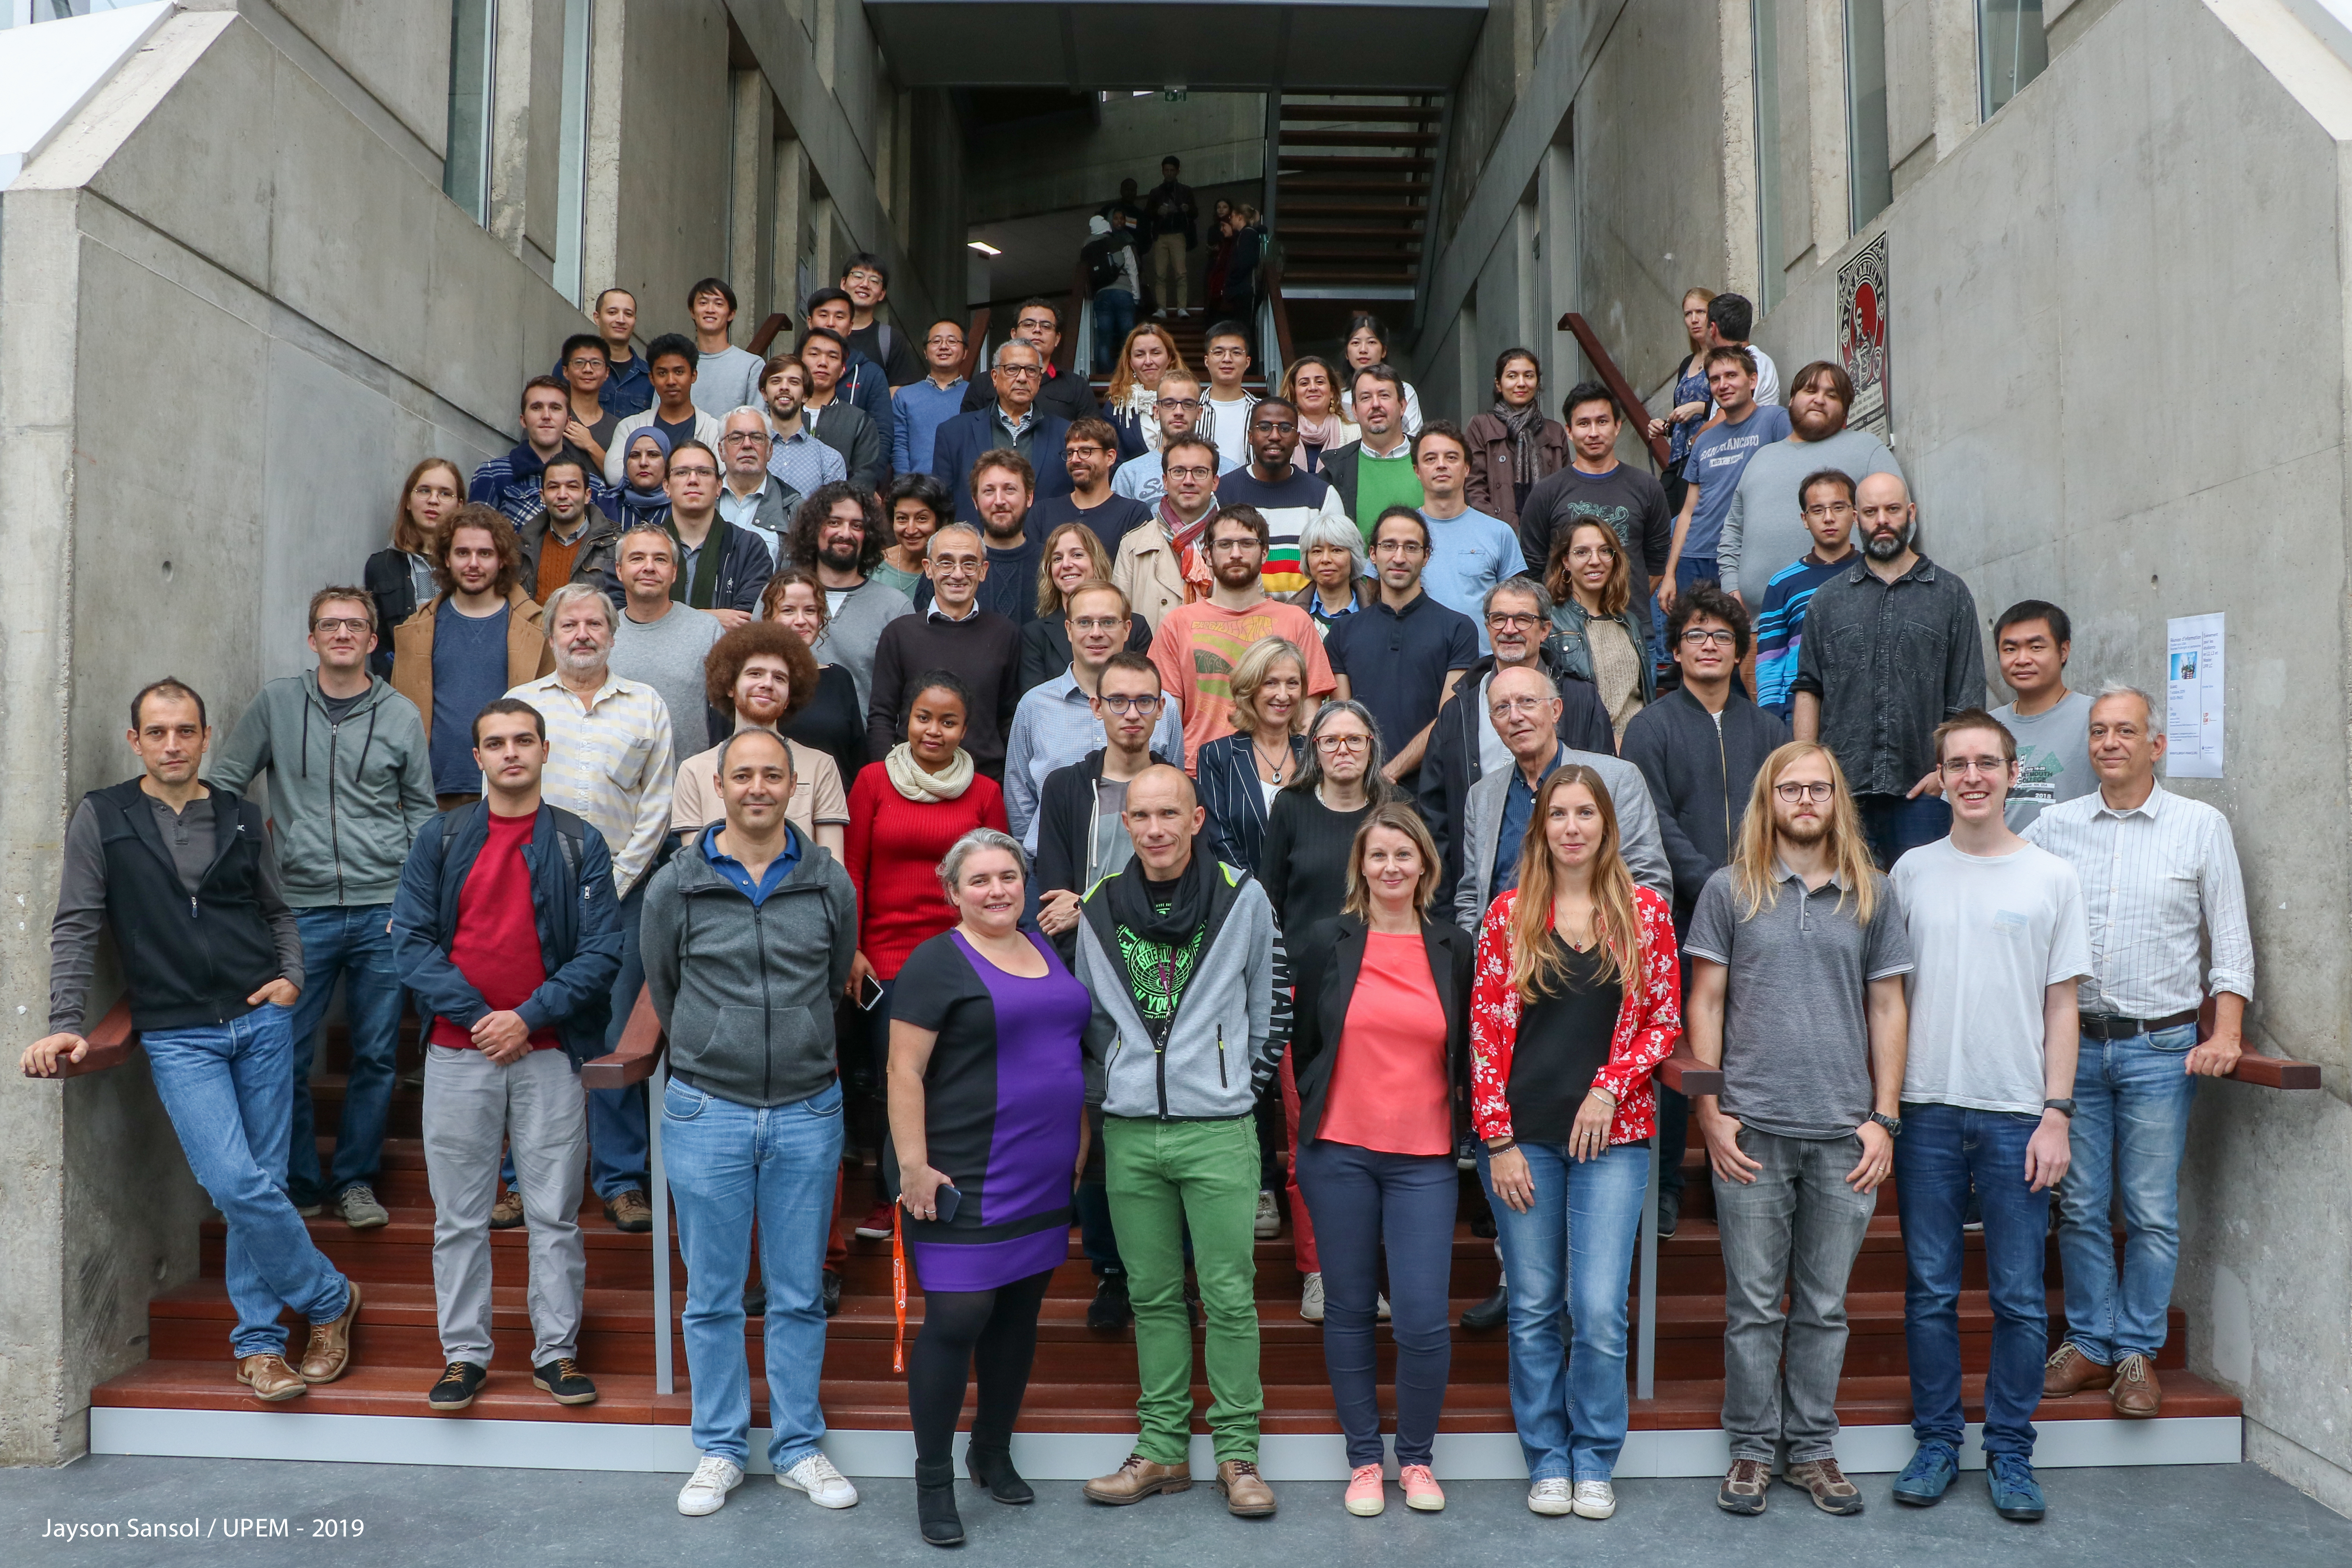
\includegraphics[scale=.22]{pictures/photo-groupe}
%   \end{center}
%
% \end{frame}
%
% %%%%%%%%%%%%%%%%%%%%%%%%%%%%%%%%%%%%%%%%%%%%%%%%%%%%%%%%%%%%%%%%%%%%%%%%%%%%%%
%
% \begin{frame}
%   \frametitle{Structure}
%
%   \begin{block}{Les équipes de recherche}
%     \begin{itemize}
%       \item \textbf{A3SI}
%
%       Algorithmes, architectures, analyse et synthèse d’images
%
%       \item \textbf{COMBI}
%
%       Combinatoire algébrique et calcul symbolique
%
%       \item \textbf{LRT}
%
%       Logiciels, réseaux et temps réel
%
%       \item \textbf{MOA}
%
%       Modèles et algorithmes
%
%       \item \textbf{SIGNAL}
%
%       Signal et communication
%     \end{itemize}
%   \end{block}
%
% \end{frame}
%
% %%%%%%%%%%%%%%%%%%%%%%%%%%%%%%%%%%%%%%%%%%%%%%%%%%%%%%%%%%%%%%%%%%%%%%%%%%%%%%
%
% \begin{frame}
%   \frametitle{Algorithmes, architectures, analyse et synthèse d’images}
%
%   \begin{block}{Direction}
%     \textsc{J.~Cousty}, ESIEE.
%   \end{block}
%
%   \begin{overprint}
%     \onslide<1>
%     \begin{block}{Effectifs (CNRS, ENPC, ESIEE \& UPEM)}
%       \begin{tabular}{ll}
%         Permanents & \fh{3}{23} \\
%         Doctorants & \fh{5}{36}  \\
%       \end{tabular}
%     \end{block}
%
%     \begin{block}{Thèmes de recheche}
%       \begin{itemize}
%         \item Architectures dédiées pour l’imagerie.
%         \item Géométrie et topologie discrètes, géométrie algorithmique.
%         \item Morphologie mathématique, filtrage et analyse d’images.
%         \item Optimisation, apprentissage et traitement d’images.
%         \item Vision artificielle.
%       \end{itemize}
%     \end{block}
%
%     \onslide<2>
%     \begin{block}{Points forts}
%       \begin{itemize}
%         \item Reconnaissance internationale.
%         \item Activité contractuelle et partenariats.
%         \item possibilités pluridisciplinaires.
%       \end{itemize}
%     \end{block}
%
%     \begin{block}{Vigilance}
%       \begin{itemize}
%         \item Nombreux départs.
%         \item Restructuration.
%       \end{itemize}
%     \end{block}
%   \end{overprint}
% \end{frame}
%
% %%%%%%%%%%%%%%%%%%%%%%%%%%%%%%%%%%%%%%%%%%%%%%%%%%%%%%%%%%%%%%%%%%%%%%%%%%%%%%
%
% \begin{frame}
%   \frametitle{Combinatoire algébrique et calcul symbolique}
%
%   \begin{block}{Direction}
%     \textsc{J.-Y.~Thibon}, UPEM.
%   \end{block}
%
%   \begin{overprint}
%     \onslide<1>
%     \begin{block}{Effectifs (CNRS \& UPEM)}
%       \begin{tabular}{ll}
%         Permanents & \fh{0}{6} \\
%         Doctorants & \fh{0}{3}  \\
%       \end{tabular}
%     \end{block}
%
%     \begin{block}{Thèmes de recheche}
%       \begin{itemize}
%         \item Algèbres de Hopf combinatoires.
%         \item Probabilités.
%         \item Combinatoire bijective et énumérative.
%         \item Opérades.
%       \end{itemize}
%     \end{block}
%
%     \onslide<2>
%     \begin{block}{Points forts}
%       \begin{itemize}
%         \item Reconnaissance internationale.
%         \item Activité éditoriale.
%       \end{itemize}
%     \end{block}
%
%     \begin{block}{Vigilance}
%       \begin{itemize}
%         \item Vivier de recrutement.
%       \end{itemize}
%     \end{block}
%   \end{overprint}
% \end{frame}
%
% %%%%%%%%%%%%%%%%%%%%%%%%%%%%%%%%%%%%%%%%%%%%%%%%%%%%%%%%%%%%%%%%%%%%%%%%%%%%%%
%
% \begin{frame}
%   \frametitle{Logiciels, réseaux et temps réel}
%
%   \begin{block}{Direction}
%     \textsc{R.~Langar}, UPEM.
%   \end{block}
%
%   \begin{overprint}
%     \onslide<1>
%     \begin{block}{Effectifs (ESIEE \& UPEM)}
%       \begin{tabular}{ll}
%         Permanents & \fh{2}{14} \\
%         Doctorants & \fh{3}{10}  \\
%       \end{tabular}
%     \end{block}
%
%     \begin{block}{Thèmes de recheche}
%       \begin{itemize}
%         \item Optimisation des ressources et contrôle d’accès dans les réseaux mobiles
%         de nouvelle génération.
%         \item Sécurité et QoS dans les réseaux sans fil.
%         \item IoT \& plateforme Java.
%         \item Ordonnancement temps-réel et efficacité énergétique.
%       \end{itemize}
%     \end{block}
%
%     \onslide<2>
%     \begin{block}{Points forts}
%       \begin{itemize}
%         \item \'Equipe en progression.
%         \item Activité contractuelle et Partenariats.
%         \item possibilités pluridisciplinaires.
%       \end{itemize}
%     \end{block}
%
%     \begin{block}{Vigilance}
%       \begin{itemize}
%         \item \'Equipe jeune.
%         \item Logiciel.
%       \end{itemize}
%     \end{block}
%   \end{overprint}
% \end{frame}
%
% %%%%%%%%%%%%%%%%%%%%%%%%%%%%%%%%%%%%%%%%%%%%%%%%%%%%%%%%%%%%%%%%%%%%%%%%%%%%%%
%
% \begin{frame}
%   \frametitle{Modèles et algorithmes}
%
%   \begin{block}{Direction}
%       \textsc{G.~Kutcherov}, CNRS.
%   \end{block}
%
%   \begin{overprint}
%     \onslide<1>
%     \begin{block}{Effectifs (ESIEE \& UPEM)}
%       \begin{tabular}{ll}
%         Permanents & \fh{7}{25} \\
%         Doctorants & \fh{1}{4}  \\
%       \end{tabular}
%     \end{block}
%
%     \begin{block}{Thèmes de recheche}
%       \begin{itemize}
%         \item Bases de données.
%         \item Automates \& logique.
%         \item Algorithmique (géométrie, analyse \& bioinformatique).
%         \item Linguistique pour le traitement automatique des langues.
%       \end{itemize}
%     \end{block}
%
%     \onslide<2>
%     \begin{block}{Points forts}
%       \begin{itemize}
%         \item Reconnaissance internationale.
%         \item Activité éditoriale.
%         \item Forte attractivité.
%       \end{itemize}
%     \end{block}
%
%     \begin{block}{Vigilance}
%       \begin{itemize}
%         \item Vivier de doctorants.
%         \item TAL.
%         \item Restructuration.
%       \end{itemize}
%     \end{block}
%   \end{overprint}
% \end{frame}
%
% %%%%%%%%%%%%%%%%%%%%%%%%%%%%%%%%%%%%%%%%%%%%%%%%%%%%%%%%%%%%%%%%%%%%%%%%%%%%%%
%
% \begin{frame}
%   \frametitle{Signal et communication}
%
%   \begin{block}{Direction}
%     \textsc{F.-X.~Vialard}, UPEM.
%   \end{block}
%
%   \begin{overprint}
%     \onslide<1>
%     \begin{block}{Effectifs (CNRS, ESIEE \& UPEM)}
%       \begin{tabular}{ll}
%         Permanents & \fh{1}{6} \\
%         Doctorants & \fh{2}{3}  \\
%       \end{tabular}
%     \end{block}
%
%     \begin{block}{Thèmes de recheche}
%       \begin{itemize}
%         \item Applications au traitement du signal en grande dimension.
%         Fluctuations locales et globales pour le spectre de grandes matrices
%         aléatoires.
%         \item Modèles non-hermitiens.
%         \item Minimisation en grande dimension et application au traitement d’images.
%         \item Transport optimal
%       \end{itemize}
%     \end{block}
%
%     \onslide<2>
%     \begin{block}{Points forts}
%       \begin{itemize}
%         \item Reconnaissance internationale.
%         \item Activité contractuelle.
%         \item Distinctions (IUF \& Prix Ac. des Sciences).
%       \end{itemize}
%     \end{block}
%
%     \begin{block}{Vigilance}
%       \begin{itemize}
%         \item Vivier de doctorants.
%         \item Départs \& disponibilités.
%       \end{itemize}
%     \end{block}
%   \end{overprint}
% \end{frame}
%
% %%%%%%%%%%%%%%%%%%%%%%%%%%%%%%%%%%%%%%%%%%%%%%%%%%%%%%%%%%%%%%%%%%%%%%%%%%%%%%
%
% \begin{frame}
%   \frametitle{Arrivées 2019}
%
%   \begin{columns}
%     \begin{column}{0.5\textwidth}
%       \begin{block}{UPEM}
%         \begin{itemize}
%           \item \textsc{F.~Reiter}, MOA.
%           \item \textsc{W.~Fang}, MOA.
%         \end{itemize}
%       \end{block}
%
%       \bigskip
%
%       \begin{block}{CNRS}
%         \begin{itemize}
%           \item \textsc{A.~de~Mesmay}, MOA.
%         \end{itemize}
%       \end{block}
%     \end{column}
%     \begin{column}{0.5\textwidth}
%       \begin{block}{ESIEE}
%         \begin{itemize}
%           \item \textsc{M.-L.~Cauwet}, SIGNAL.
%           \item \textsc{\'E.~Renault}, LRT.
%         \end{itemize}
%       \end{block}
%
%       \bigskip
%
%       \begin{block}{ENPC}
%         \begin{itemize}
%           \item \textsc{V.~Lepetit}, A3SI.
%           \item \textsc{D.~Picard}, A3SI.
%         \end{itemize}
%       \end{block}
%     \end{column}
%   \end{columns}
% \end{frame}
%
% %%%%%%%%%%%%%%%%%%%%%%%%%%%%%%%%%%%%%%%%%%%%%%%%%%%%%%%%%%%%%%%%%%%%%%%%%%%%%%
%
% \begin{frame}
%   \frametitle{Conseil de laboratoire}
%
%   \begin{block}{Membres élus}
%     \begin{columns}
%       \begin{column}{0.5\textwidth}
%         \begin{itemize}
%           \item \textsc{J.~Cousty}, ESIEE.
%           \item \textsc{S.~Giraudo}, UPEM.
%           \item \textsc{W.~Hachem}, CNRS.
%           \item \textsc{V.~Jugé}, UPEM.
%         \end{itemize}
%       \end{column}
%       \begin{column}{0.5\textwidth}
%         \begin{itemize}
%           \item \textsc{G.~Kucherov}, CNRS.
%           \item \textsc{\'E.~Laporte}, UPEM.
%           \item \textsc{C.~Palescandolo}, CNRS.
%           \item \textsc{N.~Salhab}, ESIEE.
%         \end{itemize}
%       \end{column}
%     \end{columns}
%   \end{block}
%
%   \begin{block}{Membres nommés}
%     \begin{columns}
%       \begin{column}{0.5\textwidth}
%         \begin{itemize}
%           \item \textsc{R.~Langar}, UPEM.
%           \item \textsc{P.~Monasse}, ENPC.
%         \end{itemize}
%       \end{column}
%       \begin{column}{0.5\textwidth}
%         \begin{itemize}
%           \item \textsc{J.-Y.~Thibon}, UPEM.
%           \item \textsc{F.-X.~Vialard}, UPEM.
%         \end{itemize}
%       \end{column}
%     \end{columns}
%   \end{block}
%
%   \begin{block}{Membres de droit}
%     \begin{columns}
%       \begin{column}{0.5\textwidth}
%         \begin{itemize}
%           \item \textsc{J.~Najim}, CNRS.
%         \end{itemize}
%       \end{column}
%       \begin{column}{0.5\textwidth}
%         \begin{itemize}
%           \item \textsc{S.~Vialette}, CNRS.
%         \end{itemize}
%       \end{column}
%     \end{columns}
%   \end{block}
%
% \end{frame}
%
% %%%%%%%%%%%%%%%%%%%%%%%%%%%%%%%%%%%%%%%%%%%%%%%%%%%%%%%%%%%%%%%%%%%%%%%%%%%%%%
%
% \begin{frame}
%   \frametitle{Implications}
%
%   \begin{columns}
%     \begin{column}{0.5\textwidth}
%       \begin{block}{Structure locales}
%       	\begin{itemize}
%         	\item Président de l'UPEM
%         	\item VP E. UPEM
%         	\item VP rel. int. UPEM
%         	\item Conseils centraux UPEM
%         	\item Dir. ESIEE (fin 2017)
%         	\item Dir. R. ESIEE (fin 2017)
%         	\item Directeurs du Labex
%       	\end{itemize}
%       \end{block}
%       \begin{block}{Structures régionales}
%         \begin{itemize}
%            \item Bureau DIM RFSI
%         \end{itemize}
%       \end{block}
%     \end{column}
%     \begin{column}{0.5\textwidth}
%       \begin{block}{Structures nationales}
%       	\begin{itemize}
%         	\item Président de la CPU
%         	\item Chargé mission INS2I
%         	\item CNU 27 \& 61
%         	\item Président CoNRS 41
%         	\item CoNRS 7
%         	\item Membres de comités ANR
%         	\item Dir. GDR MEGA
%         	\item Comité Dir. GDR ISIS
%         	\item Resp. GT du GDR-IM
%         	\item Comité prix Gilles Kahn
%       	\end{itemize}
%       \end{block}
%     \end{column}
%   \end{columns}
% \end{frame}
%
%
% %%%%%%%%%%%%%%%%%%%%%%%%%%%%%%%%%%%%%%%%%%%%%%%%%%%%%%%%%%%%%%%%%%%%%%%%%%%%%%
%
% \begin{frame}
%   \frametitle{Actualités récentes et échéances}
%
%   \begin{tabular}{@{\,}r <{\hskip 2pt} !{\foo} >{\raggedright\arraybackslash}p{6cm}}
%     \textbf{Novembre 2018}  & Retour déménagement phase 2 \\
%     \textbf{Janvier 2019}   & Renouvellement direction LIGM et conseil de laboratoire\\
%     \textbf{Février 2019}   & Visite Hcéres \\
%     \textbf{Mars 2019}      & Renouvellement des chefs d'équipe (A3SI, MOA et SIGNAL) \\
%     \textbf{Septembre 2019} & Retour déménagement phase 3 \\
%     \textbf{Janvier 2020}   & Université Gustave Eiffel \\
%     \textbf{Janvier-Février 2020} & Renouvellement conseil de laboratoire.
%   \end{tabular}
%
% \end{frame}
%
% %%%%%%%%%%%%%%%%%%%%%%%%%%%%%%%%%%%%%%%%%%%%%%%%%%%%%%%%%%%%%%%%%%%%%%%%%%%%%%
%
% \begin{frame}[label=introduction, standout]{}
%   Environnement scientifique
% \end{frame}
%
% %%%%%%%%%%%%%%%%%%%%%%%%%%%%%%%%%%%%%%%%%%%%%%%%%%%%%%%%%%%%%%%%%%%%%%%%%%%%%%
%
% \begin{frame}
%   \frametitle{Structures locales}
%
%   \begin{center}
%     \begin{tikzpicture}
%       \draw[fill=yellow!20,very thick, rounded corners] (0,0) rectangle (11,3.6); \node at (10.4,.3) {\textbf{UPE}};
%       %\node[anchor=west] at (0,-.5) {{\bf UPE :}  COMUE Paris-Est};
%
%       \draw[fill=red!20,very thick, rounded corners] (3.1,2.1) rectangle (5,2.9); \node at (4.2,2.5) {\textbf{ \small ESIEE}};
%       \draw[fill=red!20,very thick, rounded corners] (3.1,1.2) rectangle (5,2); \node at (4.2,1.6) {\textbf{ \small UPEM}};
%       \draw[fill=red!20,very thick, rounded corners] (.9,1.65) rectangle (2.8,2.45); \node at (1.6,2.05) {\textbf{ \small ENPC}};
%       \draw[fill=red!20,very thick, rounded corners]  (8.6,1.5) rectangle (10.4,2.3); \node at (9.5,1.9){\textbf{ \small UPEC}};
%       %\node[anchor=west] at (0,-1) {{\bf UPEC :}  Université Paris-Est Créteil};
%
%       \draw[fill=green!20,very thick, rounded corners] (.6,.5) rectangle (8,3.1); \node at (7.3,.8) {\textbf{ \small ISITE}};
%       \draw[fill=red!20,very thick, rounded corners] (3.1,2.1) rectangle (5,2.9); \node at (4.2,2.5) {\textbf{ \small ESIEE}};
%       \draw[fill=red!20,very thick, rounded corners] (3.1,1.2) rectangle (5,2); \node at (4.2,1.6) {\textbf{ \small UPEM}};
%       \draw[fill=red!20,very thick, rounded corners] (.9,1.65) rectangle (2.8,2.45); \node at (1.6,2.05) {\textbf{ \small ENPC}};
%       \draw[fill=red!20,very thick, rounded corners]  (8.6,1.5) rectangle (10.4,2.3); \node at (9.5,1.9){\textbf{ \small UPEC}};
%       %\node[anchor=west] at (0,-1.5) {{\bf ISITE :}  ISITE Future, centré sur la ville et son ingénierie};
%
%       \draw[fill=blue!20,very thick, rounded corners] (3,.6) rectangle (6,3); \node at (5.3,.85) {\textbf{ \small UGE}};
%       \draw[fill=red!20,very thick, rounded corners] (3.1,2.1) rectangle (5,2.9); \node at (4.2,2.5) {\textbf{ \small ESIEE}};
%       \draw[fill=red!20,very thick, rounded corners] (3.1,1.2) rectangle (5,2); \node at (4.2,1.6) {\textbf{ \small UPEM}};
%       \draw[fill=red!20,very thick, rounded corners] (.9,1.65) rectangle (2.8,2.45); \node at (1.6,2.05) {\textbf{ \small ENPC}};
%       \draw[fill=white,very thick, rounded corners=10] (2.4,1.65) rectangle (3.6, 2.45); \node at (3,2.05) {\textbf{ \small LIGM}};
%       \draw[fill=red!20,very thick, rounded corners]  (8.6,1.5) rectangle (10.4,2.3); \node at (9.5,1.9){\textbf{ \small UPEC}};
%       %\node[anchor=west] at (0,-2) {{\bf UGE :}  Université Gustave Eiffel};
%     \end{tikzpicture}
%   \end{center}
%
%   \begin{itemize}
%     \item
%     {\bf UPE :}  COMUE Paris-Est.
%     \item
%     {\bf ISITE :}  ISITE Future, centré sur la ville et son ingénierie.
%     \item
%     {\bf UGE :}  Université Gustave Eiffel.
%     \item
%     {\bf UPEC :}  Université Paris-Est Créteil.
%   \end{itemize}
%
% \end{frame}
%
% %%%%%%%%%%%%%%%%%%%%%%%%%%%%%%%%%%%%%%%%%%%%%%%%%%%%%%%%%%%%%%%%%%%%%%%%%%%%%%
%
% \begin{frame}
%   \frametitle{I-SITE FUTURE, UGE \& LIGM}
%
%   \begin{block}{I-SITE FUTURE}
%     \begin{itemize}
%       \item
%       Inventer la ville de demain.
%
%       \item
%       Université Paris-Est (COMUE), IFSTTAR, UPEM, ESIEE Paris, EAVT,
%       EIVP, IGN (au titre de l’ENSG) et ENPC.
%     \end{itemize}
%   \end{block}
%
%   \begin{block}{Université Gustave Eiffel (2020)}
%     \begin{itemize}
%       \item
%       Université multi-localisée sur le territoire français.
%
%       \begin{center}
%           \includegraphics[scale=.25]{pictures/carte_sitesUC.png}
%       \end{center}
%
%       \item
%       EIVP, ENSAVT, ENSG, ESIEE Paris, IFSTTAR et UPEM.
%     \end{itemize}
%   \end{block}
% \end{frame}
%
%
% %%%%%%%%%%%%%%%%%%%%%%%%%%%%%%%%%%%%%%%%%%%%%%%%%%%%%%%%%%%%%%%%%%%%%%%%%%%%%%
%
% \begin{frame}[label=donnees, standout]{}
%   Données financières
% \end{frame}
%
% %%%%%%%%%%%%%%%%%%%%%%%%%%%%%%%%%%%%%%%%%%%%%%%%%%%%%%%%%%%%%%%%%%%%%%%%%%%%%%
%
% \begin{frame}
%     \frametitle{Ressources propres}
%
%   \begin{block}{Utilisation}
%     \begin{itemize}
%       \item Gérées directement au niveau de la direction.
%       \item Utilisation à partir d'une demande motivée (utiliser prioritairement ses projets).
%       \item Des actions sont éventuellement lancées à l'automne.
%     \end{itemize}
%   \end{block}
%
%   \begin{block}{Actions spécifiques}
%     \begin{itemize}
%       \item Subvention de stages de M2/M1 (dès qu'il y a du potentiel).
%       \item Séjours courts d'été et d'automne.
%       \item Aide à la thématique TAL (financement de nombreux stagiaires).
%       (Action non reconduite.)
%     \end{itemize}
%   \end{block}
%
% \end{frame}
%
% %%%%%%%%%%%%%%%%%%%%%%%%%%%%%%%%%%%%%%%%%%%%%%%%%%%%%%%%%%%%%%%%%%%%%%%%%%%%%%
%
% \begin{frame}[fragile]
%   \frametitle{Données financières}
%
%   \begin{block}{Dotations}
%     \begin{center}
%       \includegraphics[scale=.7]{pictures/dotations.png}
%     \end{center}
%   \end{block}
%
% \end{frame}
%
% %%%%%%%%%%%%%%%%%%%%%%%%%%%%%%%%%%%%%%%%%%%%%%%%%%%%%%%%%%%%%%%%%%%%%%%%%%%%%%
%
% \begin{frame}[fragile]
%   \frametitle{Données financières}
%
%   \begin{block}{Dotations par tutelle par chercheur}
%     \begin{center}
%       \includegraphics[scale=.7]{pictures/dotations-par-chercheur.png}
%     \end{center}
%   \end{block}
%
% \end{frame}
%
% %%%%%%%%%%%%%%%%%%%%%%%%%%%%%%%%%%%%%%%%%%%%%%%%%%%%%%%%%%%%%%%%%%%%%%%%%%%%%%
%
% \begin{frame}
%   \frametitle{Point octobre 2019}
%
%   \begin{block}{UPEM}
%     \begin{itemize}
%       \item FG: $\simeq$ 32k\euro.
%       \item IG: $\simeq$ 18k\euro.
%     \end{itemize}
%   \end{block}
%
%   \begin{block}{CNRS}
%     \begin{itemize}
%       \item Dotation: $\simeq$ 12k\euro.
%       \item Total: $\simeq$ 25k\euro.
%     \end{itemize}
%   \end{block}
%
% \end{frame}
%
% %%%%%%%%%%%%%%%%%%%%%%%%%%%%%%%%%%%%%%%%%%%%%%%%%%%%%%%%%%%%%%%%%%%%%%%%%%%%%%
%
% \begin{frame}[fragile]
%   \frametitle{Contrats et partenariats (2013--2018)}
%
%   \begin{block}{Contrats}
%     Nous avons porté ou accompagné 55 contrats dont :
%     \begin{itemize}
%       \item Participation à 6 projets européens.
%       \item Participation 4 FUI.
%       \item Portage de 10 ANR Blanc \& JCJC .
%     \end{itemize}
%   \end{block}
%
%   \begin{block}{Partenaires industriels}
%     L'Oréal, Clarins, Saint-Gobain, SAFRAN, SAGEM Com, Heartflow (USA),
%     General Electric, Facebook, Adobe, Orange, Thales, Nokia, ENGIE, \dots
%   \end{block}
%
%   \begin{block}{Projets pluri-disciplinaires de l'I-SITE}
%   	\begin{itemize}
%     	\item 2 projets tremplin.
%     	\item 3 projets impulsion.
%   	\end{itemize}
%   \end{block}
%
% \end{frame}
%
% %%%%%%%%%%%%%%%%%%%%%%%%%%%%%%%%%%%%%%%%%%%%%%%%%%%%%%%%%%%%%%%%%%%%%%%%%%%%%%
%
% \begin{frame}[fragile]
%   \frametitle{Données financières}
%
%   \begin{block}{Ressources propres}
%     \begin{center}
%       \includegraphics[scale=.7]{pictures/ressources.png}
%     \end{center}
%   \end{block}
%
% \end{frame}
%
% %%%%%%%%%%%%%%%%%%%%%%%%%%%%%%%%%%%%%%%%%%%%%%%%%%%%%%%%%%%%%%%%%%%%%%%%%%%%%%
%
% \begin{frame}
%   \frametitle{UMR}
%
%   \begin{block}{Fonctionnement}
%     \begin{itemize}
%       \item Dotation ESIEE.
%       \item Interlocuteurs ENPC \& ESIEE.
%       \item Clarification des règles de fonctionnement.
%       \begin{itemize}
%         \item Missions \& matériels.
%         \item Doctorants.
%         \item Personnels permanents.
%       \end{itemize}
%     \end{itemize}
%   \end{block}
%
% \end{frame}
%
% %%%%%%%%%%%%%%%%%%%%%%%%%%%%%%%%%%%%%%%%%%%%%%%%%%%%%%%%%%%%%%%%%%%%%%%%%%%%%%
%
% \begin{frame}[label=points, standout]{}
%   Parité
% \end{frame}
%
% %%%%%%%%%%%%%%%%%%%%%%%%%%%%%%%%%%%%%%%%%%%%%%%%%%%%%%%%%%%%%%%%%%%%%%%%%%%%%%
%
% \begin{frame}
%   \frametitle{Parité}
%
%   \begin{block}{LIGM}
%     \begin{tabular}{ll}
%       EC. et C.   & \fh{13}{25} \\
%       $14\%$      & \fh{0}{39}  \\
%                   & \fh{0}{11}  \\
%       Doctorants  & \fh{11}{27} \\
%       $17\%$      & \fh{0}{27}  \\
%       Admin & \fh{3}{0} \\
%       IS    & \fh{0}{2} \\
%       IR    & \fh{1}{1}
%     \end{tabular}
%   \end{block}
%
% \end{frame}
%
% %%%%%%%%%%%%%%%%%%%%%%%%%%%%%%%%%%%%%%%%%%%%%%%%%%%%%%%%%%%%%%%%%%%%%%%%%%%%%%
%
% \begin{frame}
%   \frametitle{Parité - UPEM}
%
%   \begin{center}
%     \includegraphics[scale=.395]{pictures/upem-parite}
%   \end{center}
%
% \end{frame}
%
% %%%%%%%%%%%%%%%%%%%%%%%%%%%%%%%%%%%%%%%%%%%%%%%%%%%%%%%%%%%%%%%%%%%%%%%%%%%%%%
%
% \begin{frame}
%   \frametitle{Parité - Actions}
%
%   \begin{center}
%     \begin{columns}
%       \begin{column}{0.5\textwidth}
%         \includegraphics[scale=.375]{pictures/MESRI}
%       \end{column}
%       \begin{column}{0.5\textwidth}
%         \begin{itemize}
%           \item \textsc{P.~Gambette}, UPEM.
%           \item \textsc{S.~Vialette}, CNRS.
%         \end{itemize}
%       \end{column}
%     \end{columns}
%   \end{center}
%
% \end{frame}
%
% %%%%%%%%%%%%%%%%%%%%%%%%%%%%%%%%%%%%%%%%%%%%%%%%%%%%%%%%%%%%%%%%%%%%%%%%%%%%%%
%
% \begin{frame}
%   \frametitle{Parité - Actions}
%
%   \begin{center}
%     \begin{columns}
%       \begin{column}{0.7\textwidth}
%         \includegraphics[width=6cm]{pictures/MESRI-01}
%       \end{column}
%       \begin{column}{0.3\textwidth}
%         \begin{tabular}{cc}
%           \includegraphics[width=1cm]{pictures/MESRI-02} &
%           \includegraphics[width=1cm]{pictures/MESRI-03} \\
%           \includegraphics[width=1cm]{pictures/MESRI-04} &
%           \includegraphics[width=1cm]{pictures/MESRI-05} \\
%           \includegraphics[width=1cm]{pictures/MESRI-06} &
%           \includegraphics[width=1cm]{pictures/MESRI-07} \\
%           \includegraphics[width=1cm]{pictures/MESRI-08} &
%           \includegraphics[width=1cm]{pictures/MESRI-09} \\
%           \includegraphics[width=1cm]{pictures/MESRI-10} &
%         \end{tabular}
%       \end{column}
%     \end{columns}
%   \end{center}
%
% \end{frame}
%
% %%%%%%%%%%%%%%%%%%%%%%%%%%%%%%%%%%%%%%%%%%%%%%%%%%%%%%%%%%%%%%%%%%%%%%%%%%%%%%
%
% \begin{frame}
%   \frametitle{Expertes France (\url{https://expertes.fr/})}
%
%     \begin{center}
%       \includegraphics[width=10cm]{pictures/expertes}
%     \end{center}
%
% \end{frame}
%
% %%%%%%%%%%%%%%%%%%%%%%%%%%%%%%%%%%%%%%%%%%%%%%%%%%%%%%%%%%%%%%%%%%%%%%%%%%%%%%
%
% \begin{frame}
%   \frametitle{Parité - Actions}
%
%   \begin{block}{Brainstorming}
%     \begin{itemize}
%       \item Sensibilisation aux biais de sélection.
%       \item Affichage dédié.
%         \begin{itemize}
%           \item Règles congés maternité et parental.
%           \item Interviews anciennes doctorantes.
%           \item Collectifs de femmes dans le numérique.
%         \end{itemize}
%       \item Recensements.
%       \item Café \& échanges.
%       \item Coordination avec les structures locales \& CNRS.
%       (chartes, actions, points de contact, \dots).
%       \item \dots
%     \end{itemize}
%   \end{block}
%
% \end{frame}
%
% %%%%%%%%%%%%%%%%%%%%%%%%%%%%%%%%%%%%%%%%%%%%%%%%%%%%%%%%%%%%%%%%%%%%%%%%%%%%%%
%
% \begin{frame}[label=points, standout]{}
%   Carrières des rangs B
% \end{frame}
%
% %%%%%%%%%%%%%%%%%%%%%%%%%%%%%%%%%%%%%%%%%%%%%%%%%%%%%%%%%%%%%%%%%%%%%%%%%%%%%%
%
% \begin{frame}
%   \frametitle{Carrières des rangs B}
%
%   \begin{block}{Constats}
%     \begin{itemize}
%       \item Sur-services généralisés.
%       \item Responsabilités \& investissements.
%       \item Déficit de rangs A.
%       \item Peu de demandes de Délégation et CRCT.
%       \item Obligation de gérer des situations critiques.
%     \end{itemize}
%   \end{block}
%
% \end{frame}
%
% %%%%%%%%%%%%%%%%%%%%%%%%%%%%%%%%%%%%%%%%%%%%%%%%%%%%%%%%%%%%%%%%%%%%%%%%%%%%%%
%
% \begin{frame}
%   \frametitle{Carrières des rangs B}
%
%   \begin{block}{HDR}
%     \begin{itemize}
%       \item Aucune HDR dans l'équipe MOA sur la période d'évaluation de l'Hcéres.
%       \begin{itemize}
%         \item 17 MC UPEM.
%         \item 1 MC P7.
%         \item 4 CR CNRS.
%       \end{itemize}
%     \end{itemize}
%   \end{block}
%
%   \begin{block}{Composantes d'enseignement}
%     \begin{itemize}
%       \item Les directions des 3 composantes d'enseignement UPEM
%       sont assurées par des rangs B.
%       \begin{itemize}
%         \item IGM. \textsc{S.~Midonnet}, MC, UPEM.
%         \item ESIPE. \textsc{E.~Duris}, MC, UPEM.
%         \item IUT MLV. \textsc{\'E.~Incerti}, MC, UPEM.
%       \end{itemize}
%     \end{itemize}
%   \end{block}
%
% \end{frame}
%
% %%%%%%%%%%%%%%%%%%%%%%%%%%%%%%%%%%%%%%%%%%%%%%%%%%%%%%%%%%%%%%%%%%%%%%%%%%%%%%
%
% \begin{frame}
%   \frametitle{Carrières des rangs B}
%
%   \begin{block}{Actions}
%     \begin{itemize}
%       \item \'Etat des lieux (ESIEE \& UPEM).
%       \begin{itemize}
%         \item Entretiens.
%         \item Discussions UPEM \& composantes d'enseignement.
%       \end{itemize}
%       \item Accompagner \& orienter.
%       \item Encourager \& accompagner les demandes de Délégation et CRCT.
%     \end{itemize}
%   \end{block}
% \end{frame}
%
% %%%%%%%%%%%%%%%%%%%%%%%%%%%%%%%%%%%%%%%%%%%%%%%%%%%%%%%%%%%%%%%%%%%%%%%%%%%%%%
%
% \begin{frame}[label=points, standout]{}
%   LIGM \& UMR
% \end{frame}
%
% %%%%%%%%%%%%%%%%%%%%%%%%%%%%%%%%%%%%%%%%%%%%%%%%%%%%%%%%%%%%%%%%%%%%%%%%%%%%%%
%
% \begin{frame}
%   \frametitle{\'Ecole Doctorale MSTIC~--~2019}
%
%   \begin{block}{$2 \times 1/2$ allocations ENPC}
%     \begin{itemize}
%       \item
%       A3SI. \textsc{D.~Picard}, ENPC.
%     \end{itemize}
%   \end{block}
%
%   \medskip
%
%   \begin{block}{$2 \times 1/2$ allocations ESIEE}
%     \begin{itemize}
%       \item
%       LRT. \textsc{L.~George}, ESIEE \& \textsc{A.~Badis}, UPEM.
%     \end{itemize}
%   \end{block}
%
%   \medskip
%
%   \begin{block}{$9 \times 1$ allocations UPEM}
%     \begin{itemize}
%       \item
%       COMBI. \textsc{J.-C.~Novelli}, UPEM.
%       \item
%       A3SI. \textsc{P.~Monasse}, ENPC \& \textsc{V.~Nozick}, UPEM.
%       \item
%       A3SI. \textsc{E.~Dokladalova}, ESIEE \& \textsc{P.~Monasse}, ENPC.
%     \end{itemize}
%   \end{block}
%
% \end{frame}
%
% %%%%%%%%%%%%%%%%%%%%%%%%%%%%%%%%%%%%%%%%%%%%%%%%%%%%%%%%%%%%%%%%%%%%%%%%%%%%%%
%
% \begin{frame}
%   \frametitle{Affiliations}
%
%   \begin{center}
%     \includegraphics[scale=.355]{pictures/disorders-permutations}
%   \end{center}
% \end{frame}
%
% %%%%%%%%%%%%%%%%%%%%%%%%%%%%%%%%%%%%%%%%%%%%%%%%%%%%%%%%%%%%%%%%%%%%%%%%%%%%%%
%
% \begin{frame}[fragile]
%   \frametitle{UMR}
%
%   \begin{block}{Quelques messages}
%     {\footnotesize
%       \begin{verbatim}
% Bonsoir Stéphane,
% Question peut être stupide :-) la gratification de stage c'est que
% pour les membres de l'UPEM?
%       \end{verbatim}
%     }%
%
%     {\footnotesize
%       \begin{verbatim}
% Sachant que l'ESIEE fourni déjà des locaux pour nos stagiaires,
% est-ce que tu penses que le LIGM aurait un financement pour remplacer
% 2 à 4 machines?
%       \end{verbatim}
%     }%
%
%     {\footnotesize
%       \begin{verbatim}
% Est-ce que quelqu'un de l'ESIEE à le droit à un support du CNRS?
%       \end{verbatim}
%     }%
%   \end{block}
%
% \end{frame}
%
% %%%%%%%%%%%%%%%%%%%%%%%%%%%%%%%%%%%%%%%%%%%%%%%%%%%%%%%%%%%%%%%%%%%%%%%%%%%%%%
%
% \begin{frame}[label=introduction, standout]{}
%   Politique scientifique et perspectives
% \end{frame}
%
% %%%%%%%%%%%%%%%%%%%%%%%%%%%%%%%%%%%%%%%%%%%%%%%%%%%%%%%%%%%%%%%%%%%%%%%%%%%%%%
%
% \begin{frame}
%   \frametitle{Politique scientifique}
%
%   \begin{block}{Visibilité et attractivité}
%     \begin{itemize} \setlength\itemsep{0em}
%       \item Exigence scientifique.
%       \item Travail avec les composantes d'enseignement.
%       \item Aide aux candidats extérieurs.
%       \item Soutien aux manifestations.
%       \item Implication dans les instances.
%       \item Soutien dans la vie de tous les jours, les carrières.
%     \end{itemize}
%   \end{block}
%
% \end{frame}
%
% %%%%%%%%%%%%%%%%%%%%%%%%%%%%%%%%%%%%%%%%%%%%%%%%%%%%%%%%%%%%%%%%%%%%%%%%%%%%%%
%
% \begin{frame}
%   \frametitle{Politique scientifique}
%
%   \begin{block}{Internationalisation}
%     \begin{itemize}
%       \item Recrutements d'étrangers.
%       \item Participation à des masters internationaux et des écoles.
%       \item Financements de visites de recherche.
%     \end{itemize}
%   \end{block}
%
%   \begin{block}{Développement des interactions au sein du Labex}
%     \begin{itemize}
%       \item Des liens très forts se sont créés avec le LAMA.
%       \item Développement de la thématique ``\emph{géométrie}'' de MOA.
%       \item Montage d'un Master Math-Info (dans le projet EUR).
%     \end{itemize}
%   \end{block}
%
% \end{frame}
%
% %%%%%%%%%%%%%%%%%%%%%%%%%%%%%%%%%%%%%%%%%%%%%%%%%%%%%%%%%%%%%%%%%%%%%%%%%%%%%%
%
% \begin{frame}
%   \frametitle{Perspectives}
%
%   \begin{block}{\'Elément clés}
%     \begin{itemize}
%       \item Fonctionnement UMR.
%       \item UGE.
%       \item ERC \& IUF.
%       \item Renforcer les équipes et excellence scientifique.
%       \item Restructuration des équipes A3SI et MOA.
%       \item Actions ATER.
%       \item Parité.
%       \item Traitement automatique des langues.
%     \end{itemize}
%   \end{block}
%
% \end{frame}
%
% %%%%%%%%%%%%%%%%%%%%%%%%%%%%%%%%%%%%%%%%%%%%%%%%%%%%%%%%%%%%%%%%%%%%%%%%%%%%%%
%
% \begin{frame}
%   \frametitle{Perspectives}
%
%   \begin{block}{Développement logiciel - Bilan}
%     \begin{itemize}
%       \item Nombreux développements logiciels au sein du LIGM.
%       \item \'Enormes besoins en développement logiciel (A3SI, LRT, \dots).
%       \item Solutions ad hoc non pérennes.
%       \item Véritable culture du développement logiciel.
%       \item Le LIGM développe une politique de référencement et de valorisation logicielle.
%     \end{itemize}
%   \end{block}
%
%   \begin{block}{Développement logiciel - Projet}
%     \begin{itemize}
%       \item Mutualisation.
%       \item Actions coordonnées des tutelles.
%       \item I-SITE FUTURE \& UGE.
%     \end{itemize}
%   \end{block}
%
% \end{frame}
%
% %%%%%%%%%%%%%%%%%%%%%%%%%%%%%%%%%%%%%%%%%%%%%%%%%%%%%%%%%%%%%%%%%%%%%%%%%%%%%%
%
% \section*{Annexes}
%
% %%%%%%%%%%%%%%%%%%%%%%%%%%%%%%%%%%%%%%%%%%%%%%%%%%%%%%%%%%%%%%%%%%%%%%%%%%%%%%
%
% \begin{frame}[label=conclusion, standout]{Annexes}
%   Effectifs
% \end{frame}
%
% %%%%%%%%%%%%%%%%%%%%%%%%%%%%%%%%%%%%%%%%%%%%%%%%%%%%%%%%%%%%%%%%%%%%%%%%%%%%%%
%
% \begin{frame}
%   \frametitle{Algorithmes, architectures, analyse et synthèse d’images}
%
%   \begin{block}{Effectifs}
%     \begin{overprint}
%       \onslide<1>
%       \begin{columns}
%         \begin{column}{0.5\textwidth}
%           \begin{itemize}
%             \item \textsc{M.~Akil}, ESSIE
%             \item \textsc{M.~Aubry}, ENPC
%             \item \textsc{S.~Berraf}, ESSIE
%             \item \textsc{G.~Bertrand}, ESSIE
%             \item \textsc{V.~Biri}, UPEM
%             \item \textsc{L.~Buzer}, ESSIE
%             \item \textsc{G.~Chierchia}, ESSIE
%           \end{itemize}
%         \end{column}
%         \begin{column}{0.5\textwidth}
%           \begin{itemize}
%             \item \textsc{C.~Chu}, ESSIE
%             \item \textsc{M.~Couprie}, ESIEE
%             \item \alert{\textsc{J.~Cousty}, ESIEE}
%             \item \textsc{E.~Dokladalova}, ESSIE
%             \item \textsc{T.~Grandpierre}, ESSIE
%             \item \textsc{R.~Jeansoulin}, CNRS
%           \end{itemize}
%         \end{column}
%       \end{columns}
%
%       \onslide<2>
%       \begin{columns}
%         \begin{column}{0.5\textwidth}
%           \begin{itemize}
%             \item \textsc{R.~Kachouri}, ESIEE
%             \item \textsc{Y.~Kenmochi}, CNRS
%             \item \textcolor{Nouveau}{\textsc{V.~Lepetit}, ENPC}
%             \item \textsc{R.~Marlet}, ENPC
%             \item \textsc{P.~Monasse}, ENPC
%             \item \textsc{N.~Mustafa}, ESIEE
%             \item \textsc{L.~Najman}, ESIEE
%           \end{itemize}
%         \end{column}
%         \begin{column}{0.5\textwidth}
%           \begin{itemize}
%             \item \textsc{B.~Neveu}, ENPC
%             \item \textsc{V.~Nozick}, UPEM
%             \item \textsc{B.~Perret}, ESIEE
%             \item \textsc{D.~Picard}, ENPC
%             \item \textsc{A.~Sahli}, ESIEE
%             \item \textsc{C.~Wang}, UPEM
%           \end{itemize}
%         \end{column}
%       \end{columns}
%     \end{overprint}
%   \end{block}
% \end{frame}
%
% %%%%%%%%%%%%%%%%%%%%%%%%%%%%%%%%%%%%%%%%%%%%%%%%%%%%%%%%%%%%%%%%%%%%%%%%%%%%%%
%
% \begin{frame}
%   \frametitle{Combinatoire algébrique et calcul symbolique}
%
%   \begin{block}{Effectifs}
%       \begin{columns}
%         \begin{column}{0.5\textwidth}
%           \begin{itemize}
%             \item \textsc{P.~Biane}, CNRS
%             \item \textsc{N.~Borie}, UPEM
%             \item \textsc{O.~Bouillot}, UPEM
%             \item \textsc{S.~Giraudo}, UPEM
%           \end{itemize}
%         \end{column}
%
%         \begin{column}{0.5\textwidth}
%           \begin{itemize}
%             \item \textsc{J.-C.~Novelli}, UPEM
%             \item \alert{\textsc{J.-Y.~Thibon}, UPEM}
%             \item \textsc{F.~Toumazet}, UPEM
%           \end{itemize}
%         \end{column}
%       \end{columns}
%   \end{block}
% \end{frame}
%
% %%%%%%%%%%%%%%%%%%%%%%%%%%%%%%%%%%%%%%%%%%%%%%%%%%%%%%%%%%%%%%%%%%%%%%%%%%%%%%
%
% \begin{frame}
%   \frametitle{Modèles et algorithmes}
%
%   \begin{block}{Effectifs}
%     \begin{overprint}
%       \onslide<1>
%       \begin{columns}
%         \begin{column}{0.5\textwidth}
%           \begin{itemize}
%             \item \textsc{M.-P.~Béal}, UPEM
%             \item \textsc{L.~Bulteau}, CNRS
%             \item \textsc{A.~Carayol}, CNRS
%             \item \textsc{D.~Caucal}, CNRS
%             \item \textsc{\'E.~Colin De V.}, CNRS
%             \item \textsc{M.~Crochemore}, UPEM
%             \item \textsc{O.~Curé}, UPEM
%             \item \textsc{C.~David}, UPEM
%           \end{itemize}
%         \end{column}
%
%         \begin{column}{0.5\textwidth}
%           \begin{itemize}
%             \item \textsc{I.~Fagnot}, P7
%             \item \textcolor{Nouveau}{\textsc{W.~Fang}, UPEM}
%             \item \textsc{N.~Francis}, UPEM
%             \item \textsc{P.~Gambette}, UPEM
%             \item \textsc{A.~Hubard}, UPEM
%             \item \textsc{V.~Jugé}, UPEM
%             \item \alert{\textsc{G.~Kucherov}, CNRS}
%             \item \textsc{T.~Kyriacopoulou}, UPEM
%           \end{itemize}
%         \end{column}
%       \end{columns}
%
%       \onslide<2>
%       \begin{columns}
%         \begin{column}{0.5\textwidth}
%           \begin{itemize}
%             \item \textsc{A.~Labarre}, UPEM
%             \item \textsc{\'E.~Laporte}, UPEM
%             \item \textsc{V.~Marsault}, CNRS
%             \item \textcolor{Nouveau}{\textsc{A.~de~Mesmay}, CNRS}
%             \item \textsc{A.~Meyer}, UPEM
%             \item \textsc{T.~Nakamura}, CNRS
%             \item \textsc{C.~Nicaud}, UPEM
%             \item \textsc{D.~Perrin}, UPEM
%             \item \textsc{C.~Pivoteau}, UPEM
%           \end{itemize}
%         \end{column}
%         \begin{column}{0.5\textwidth}
%           \begin{itemize}
%             \item \textcolor{Nouveau}{\textsc{F.~Reiter}, UPEM}
%             \item \textsc{D.~Revuz}, UPEM
%             \item \textsc{G.~Rindone}, UPEM
%             \item \textsc{C.~Rispal}, UPEM
%             \item \textsc{J.~Thapper}, UPEM
%             \item \textsc{S.~Vialette}, CNRS
%             \item \textsc{M.~Weller}, CNRS
%           \end{itemize}
%         \end{column}
%       \end{columns}
%     \end{overprint}
%   \end{block}
% \end{frame}
%
% %%%%%%%%%%%%%%%%%%%%%%%%%%%%%%%%%%%%%%%%%%%%%%%%%%%%%%%%%%%%%%%%%%%%%%%%%%%%%%
%
% \begin{frame}
%   \frametitle{Logiciels, réseaux et temps réel}
%
%   \begin{block}{Effectifs}
%     \begin{columns}
%       \begin{column}{0.5\textwidth}
%         \begin{itemize}
%           \item \textsc{Y.~Abdeddaïm}, ESIEE
%           \item \textsc{N.~Ait Saadi}, ESIEE
%           \item \textsc{H.~Badis}, UPEM
%           \item \textsc{S.~Cherrier}, UPEM
%           \item \textsc{E.~Duris}, UPEM
%           \item \textsc{R.~Forax}, UPEM
%           \item \textsc{L.~George}, ESIEE
%           \item \alert{\textsc{R.~Langar}, UPEM}
%         \end{itemize}
%       \end{column}
%       \begin{column}{0.5\textwidth}
%         \begin{itemize}
%           \item \textsc{S.~Lohier}, UPEM
%           \item \textsc{D.~Masson}, ESIEE
%           \item \textsc{S.~Midonnet}, UPEM
%           \item \textsc{A.~Rachedi}, UPEM
%           \item \textcolor{Nouveau}{\textsc{\'E.~Renault}, ESIEE}
%           \item \textsc{G.~Roussel}, UPEM
%           \item \textsc{T.~Wang}, ESIEE
%           \item \textsc{N.~Zangar}, ESIEE
%         \end{itemize}
%       \end{column}
%     \end{columns}
%   \end{block}
%
% \end{frame}
%
% %%%%%%%%%%%%%%%%%%%%%%%%%%%%%%%%%%%%%%%%%%%%%%%%%%%%%%%%%%%%%%%%%%%%%%%%%%%%%%
%
% \begin{frame}
%   \frametitle{Signal et communication}
%
%   \begin{block}{Effectirfs}
%     \begin{columns}
%       \begin{column}{0.5\textwidth}
%         \begin{itemize}
%           \item \textsc{J.-F.~Bercher}, ESIEE
%           \item \textcolor{Nouveau}{\textsc{M.-L.~Cauwet}, ESIEE}
%           \item \textsc{A.~Chevreuil}, UPEM
%           \item \textsc{W.~Hachem}, CNRS
%         \end{itemize}
%       \end{column}
%       \begin{column}{0.5\textwidth}
%         \begin{itemize}
%           \item \textsc{P.~Loubaton}, UPEM
%           \item \textsc{J.~Najim}, CNRS
%           \item \alert{\textsc{F.-X.~Vialard}, UPEM}
%         \end{itemize}
%       \end{column}
%     \end{columns}
%   \end{block}
% \end{frame}
%
% %%%%%%%%%%%%%%%%%%%%%%%%%%%%%%%%%%%%%%%%%%%%%%%%%%%%%%%%%%%%%%%%%%%%%%%%%%%%%%
%
% \begin{frame}[label=conclusion, standout]{Annexes}
%   Publications
% \end{frame}
%
% %%%%%%%%%%%%%%%%%%%%%%%%%%%%%%%%%%%%%%%%%%%%%%%%%%%%%%%%%%%%%%%%%%%%%%%%%%%%%%
%
% \begin{frame}
%   \frametitle{Publications}
%
%   \begin{block}{2013--2018}
%   	\begin{center}
%     	{\small%
%     		\begin{tabular}{@{}lccccccc@{}}
%       		\toprule
%       		 & 2013 & 2014 & 2015 & 2016 & 2017 & 2018$^*$ & Total \\
%       		\midrule
%       		Journaux & 78 & 79 & 74 & 86 & 80 & 58 & 455 \\
%       		Actes conf. & 127 & 95 & 115 & 102 & 91 & 54 & 584 \\
%       		Actes work. & 16 & 18 & 14 & 19 & 14 & 12 & 93 \\
%       		Articles synthèse & 1 & 3 & 3 & 0 & 1 & 2 & 10 \\
%       		Dir. ouvrages & 3& 2& 0& 1& 0& 0& 6 \\
%       		Chap. ouvrages & 13 & 7 & 4 & 2 & 6 & 2 & 34 \\
%       		\'Edition d'acte s & 2 &  3 & 1 & 0 & 1 & 0 & 7 \\
%       		\midrule
%       		Total &240& 207& 211& 210& 193& 128& 1189 \\
%       		\bottomrule
%     		\end{tabular}
%       }% end small
%   	\end{center}
%   \end{block}
%
% \end{frame}
%
% %%%%%%%%%%%%%%%%%%%%%%%%%%%%%%%%%%%%%%%%%%%%%%%%%%%%%%%%%%%%%%%%%%%%%%%%%%%%%%
%
% \begin{frame}[label=conclusion, standout]{Annexes}
%   Données financières
% \end{frame}
%
% %%%%%%%%%%%%%%%%%%%%%%%%%%%%%%%%%%%%%%%%%%%%%%%%%%%%%%%%%%%%%%%%%%%%%%%%%%%%%%
%
% \begin{frame}
%   \frametitle{Données financières}
%
%   \begin{block}{Dotations}
%     {\footnotesize
%       \begin{center}
%         \begin{tabular}{lrrrrrrr}
%           \toprule
%           Tutelle & 2013 &  2014 & 2015 & 2016 & 2017 & S018 & 2019 \\
%           \midrule
%           CNRS    & \num{52000}  & \num{55000}  & \num{55000}  & \num{55000}  & \num{55000}  & \num{65000}  & \num{75000}  \\
%           UPEM    & \num{280520} & \num{220000} & \num{187500} & \num{236481} & \num{198500} & \num{141000} & \num{154000} \\
%           ESIEE   & \num{24500}  & \num{29000}  & \num{25500}  & \num{19950}  & \num{23450}  & \num{23450}  & \num{14350}  \\
%           ENPC    & \num{20000}  & \num{20000}  & \num{0}      & \num{0}      & \num{0}      & \num{0}      & \num{0}      \\
%           \bottomrule
%         \end{tabular}
%       \end{center}
%     }% end footnotesize
%   \end{block}
%
% \end{frame}
%
% %%%%%%%%%%%%%%%%%%%%%%%%%%%%%%%%%%%%%%%%%%%%%%%%%%%%%%%%%%%%%%%%%%%%%%%%%%%%%%
%
% \begin{frame}
%   \frametitle{Données financières}
%
%   \begin{block}{Ressources propres}
%     {\footnotesize
%       \begin{center}
%         \begin{tabular}{lrrrrrrr}
%           \toprule
%           Tutelle & 2013 &  2014 & 2015 & 2016 & 2017 & 2018 & 2019 \\
%           \midrule
%           CNRS    & \num{0}      & \num{0}      & \num{0}      & \num{0}      & \num{41307}  & \num{0} & \num{0} \\
%           UPEM    & \num{879242} & \num{846864} & \num{847588} & \num{385092} & \num{339281} & \num{474352} & \num{498368} \\
%           ESIEE   & \num{347873} & \num{449994} & \num{225541} & \num{231036} & \num{317037} & \num{257924} & \num{226500} \\
%           ENPC    & \num{486367} & \num{212681} & \num{330884} & \num{244472} & \num{238414} & \num{154892} & \num{280071} \\
%           \bottomrule
%         \end{tabular}
%       \end{center}
%     }% end footnotesize
%   \end{block}
%
% \end{frame}

%%%%%%%%%%%%%%%%%%%%%%%%%%%%%%%%%%%%%%%%%%%%%%%%%%%%%%%%%%%%%%%%%%%%%%%%%%%%%%

%%%%%%%%%%%%%%%%%%%%%%%%%%%%%%%%%%%%%%%%%%%%%%%%%%%%%%%%%%%%%%%%%%%%%%%%%%%%%%

\end{document}

%%%%%%%%%%%%%%%%%%%%%%%%%%%%%%%%%%%%%%%%%%%%%%%%%%%%%%%%%%%%%%%%%%%%%%%%%%%%%%
